\iffalse
\begin{figure}[h]
\centering
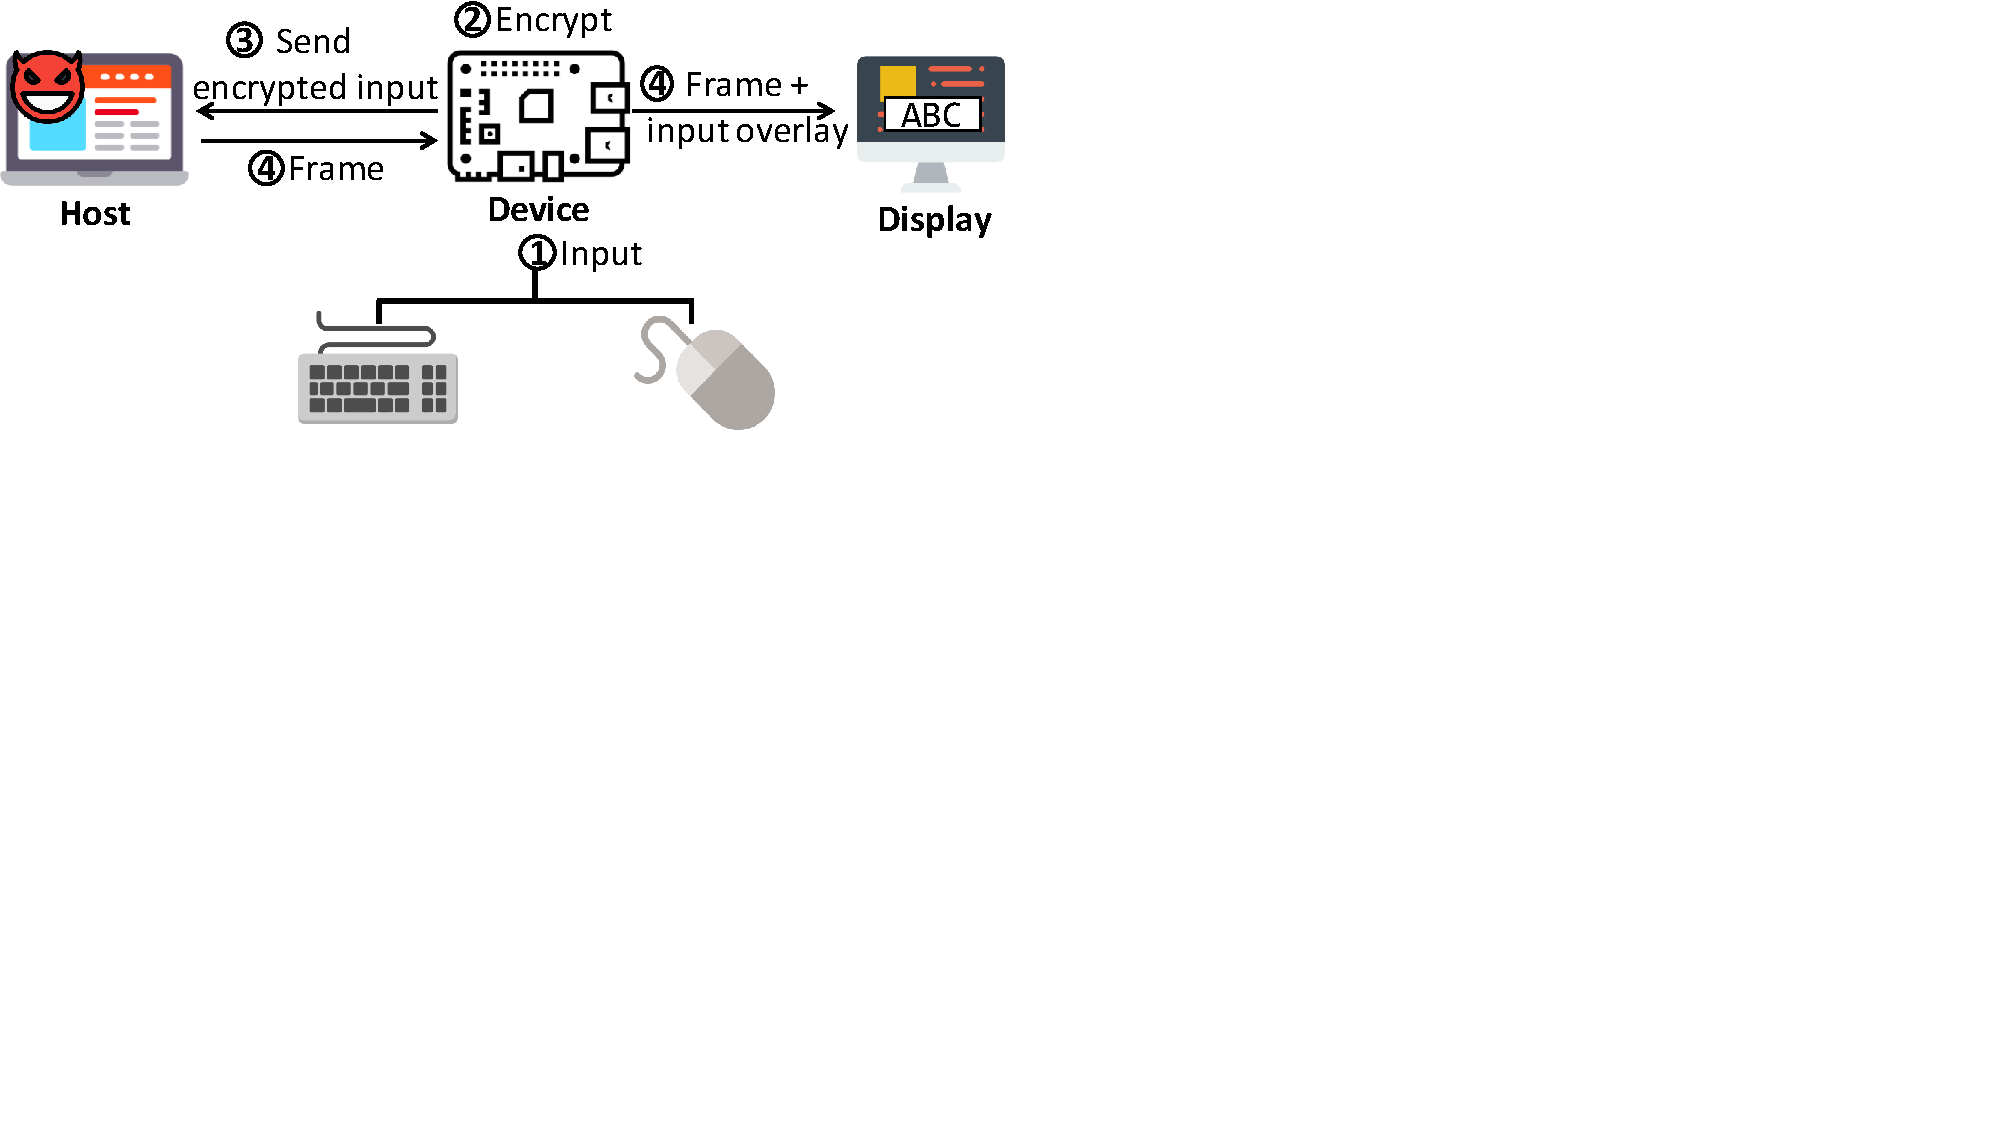
\includegraphics[trim={0 11cm 16.5cm 0}, clip, width=\linewidth]{inputPrivacy.pdf}
\caption{Input Confidentiality}
\label{fig:inputPrivacy}
\centering
\end{figure}
\fi



\section{\name for IO Confidentiality}
\label{sec:confidentiality}


In the previous sections, we describe how the \name \js and the \device together ensure the integrity of the IO. We now augment the design of \name achieve IO confidentiality alongside of the IO integrity. One of the major components for achieving IO confidentiality is to establish a secure channel (i.e., a \tls channel) between the remote server and the \device. \tls ensures that all the IO data between the user and the remote server is hidden from the untrusted host.  


\subsection{IO Operations}
\label{sec:confidentiality:io}

\lstset{language=HTML, frame=tb, caption=\small{\textbf{HTML page from the remote server that contains the encrypted UI specification for IO confidentiality.}} , label = snippet:encryptedHTML, firstnumber =1}
\begin{figure}[t]
\small
\begin{lstlisting}[mathescape=true]
<form action="/some_action">
  Text box 1:<br>
  <input type="text" name="text_box_1">
  <br> text box 2:<br>
  <input type="text" name="text_box_2">
  <encrypted_qr><!-encrypted UI specification->
  0x4a5c4... </encrypted_qr>
  <script> [JS outputs QR code that encodes 
  encrypted specification] </script>
</form> 
\end{lstlisting} 
\end{figure}



\begin{figure}[t]
\centering
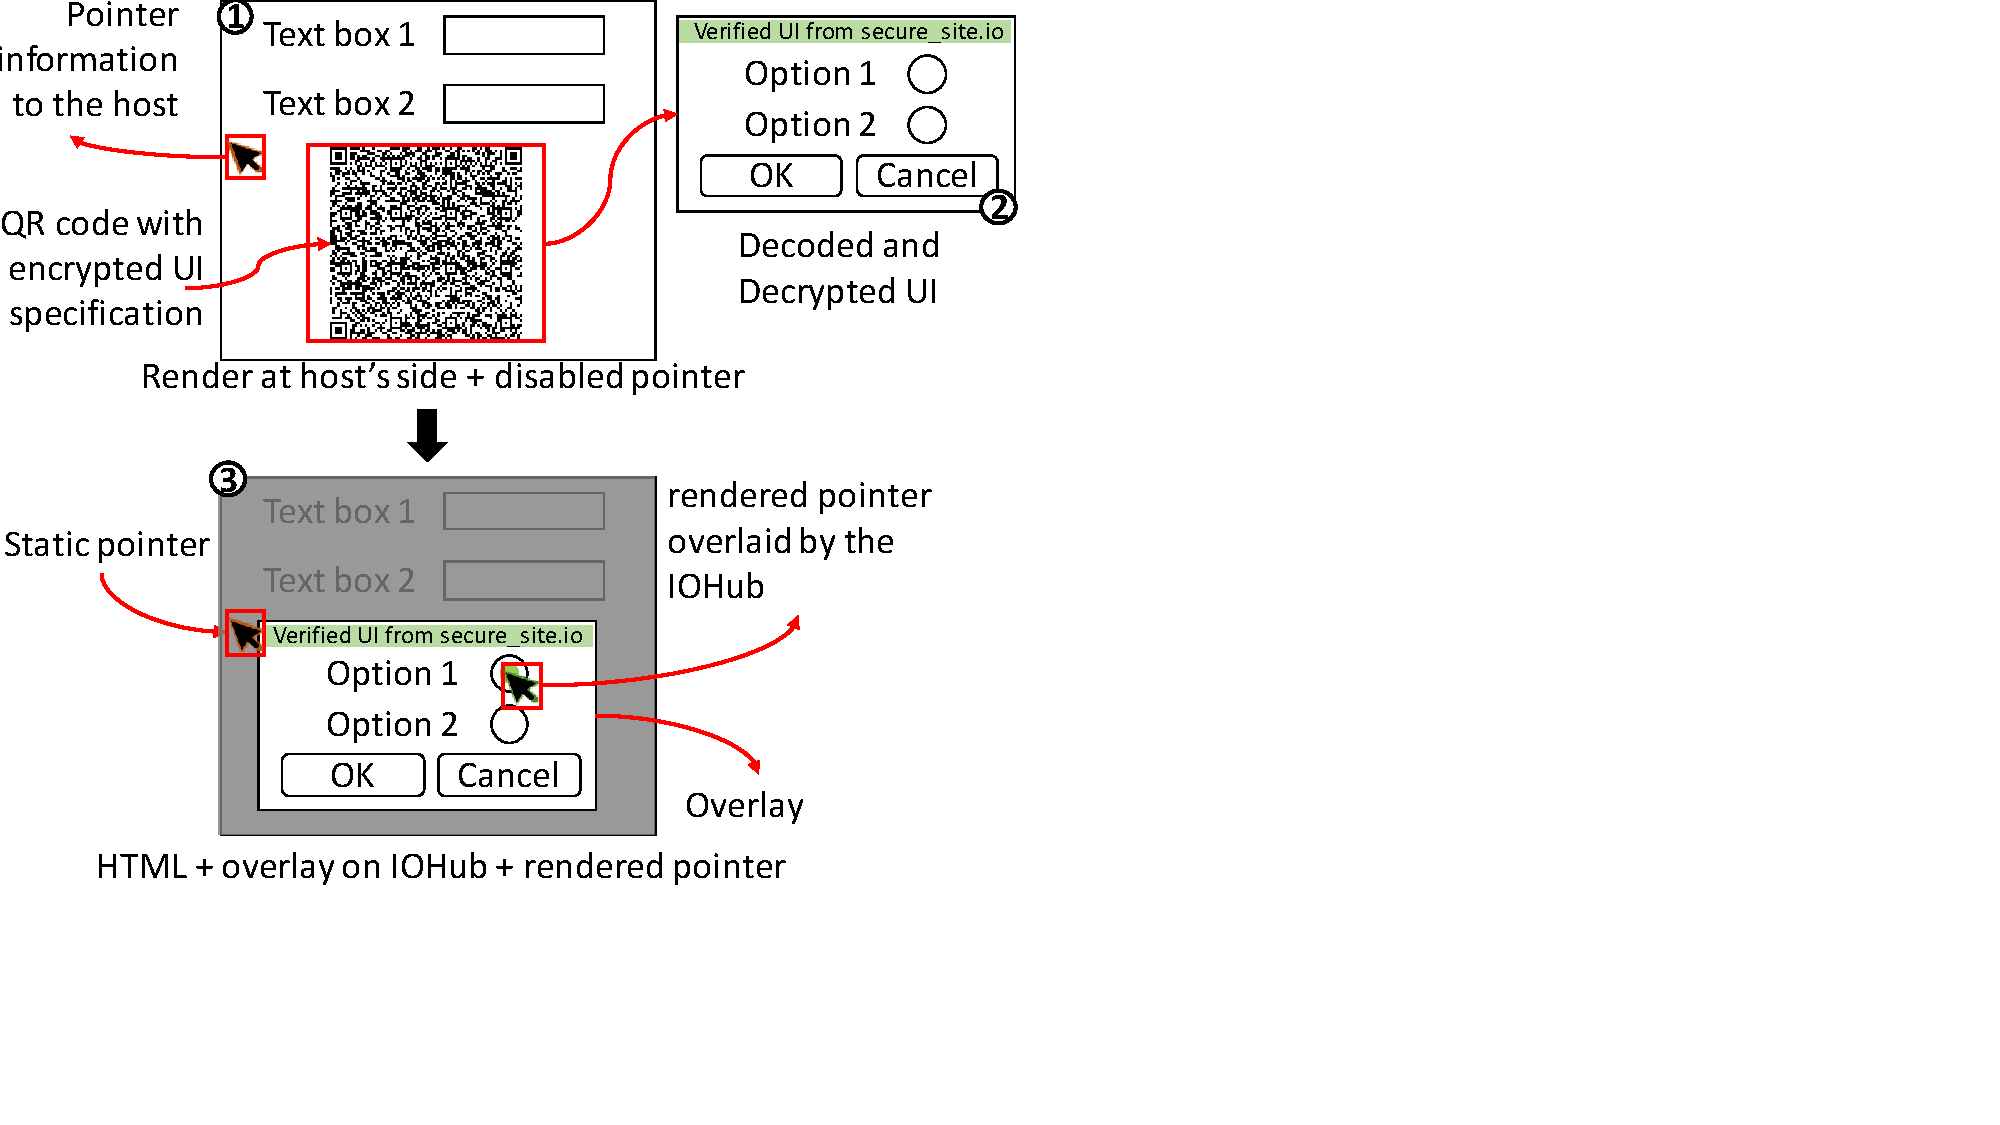
\includegraphics[trim={0 3cm 16.5cm 0}, clip, width=0.88\linewidth]{activityPrivacyRender.pdf}
%\caption{\textbf{\name IO confidentiality.} The figure shows how \name achieves the confidentiality of the UI elements and the mouse pointer in the presence of a compromised host. The upper screenshot shows the host's view of the display while the lower one shows the user's view. The host can only see a QR code where the specification is encrypted by the \tls session key between the \device and the remote server. The user saw the decoded and overlaid UI objects that are retrieved from the QR code sent by the remote server (as described in Section~\ref{sec:systemDesign:transformation}).}
\caption{\textbf{\name IO confidentiality.} The figure shows \one the browser render of the webpage in Specification~\ref{snippet:encryptedHTML} where the \name \js produce the encrypted QR code. \two shows the UI overlay that is decrypted and decoded by the \device. \three shows the user's view when the \device overlays the UI on the HDMI frame and the user starts to interact with the UI.}

\spacesave
\label{fig:activityPrivacy}
\centering
\end{figure}

After the server and the \device establish the \tls channel (we describe the technical details of the \tls channel in the next section, Section~\ref{sec:confidentiality:tls}), \name is ready to provide IO confidentiality.

\myparagraph{Output confidentiality} Output confidentiality ensures that information sent from the remote server and the UI feedback to the user's input is hidden from the host. To enable output confidentiality, the UI overlay mechanism that is described in Section~\ref{sec:systemDesign:transformation} is modified slightly. Here we \name does not require \name JS to transform all the UI elements to QR code specification. A small server-side module that is very similar to \name JS transforms the UI elements to the UI specification (one such specification is provided in Specification~\ref{snippet:UISpecification}) and encrypt the specification with the \tls session key (refer to Section~\ref{sec:confidentiality:tls}). The \device decodes the QR code from the intercepted HDMI frames, decrypts the specification and overlays the UI on the HDMI frames. One example is provided in the HTML Snippet~\ref{snippet:encryptedHTML}. The corresponding UI is illustrated in Figure~\ref{fig:activityPrivacy}. The \texttt{<encrypted>} tag contains the encrypted UI specification from the server. The \name JS (inside \texttt{<script>} tag) encodes this encrypted UI specification to a QR code.

\myparagraph{Input Confidentiality} When the user enters her mouse pointer into the overlaid UI boundary, the \device stops transmitting any mouse and keyboard signal, making the host completely oblivious to any mouse movement or keystrokes during that time. Likewise, when the user selects a UI element, for example, a radio button that is shown in Figure~\ref{fig:activityPrivacy}, the \device encrypts and signs the packets and sends the packet to the remote server making the input commands/values hidden from the attacker-controlled host. However, the user can still her input on the screen as the \device overlays the paintext character on the overlaid UI elements, making them visible only to the user. 

\myparagraph{SAS for confidentiality} Secure Attention Sequence (SAS) is a sequence of actions\footnote{Such as keystrokes \texttt{Ctrl+Alt+Del} that allows the user to provide her credential.} executed by the user that is completely trustworthy. SAS prevents an untrusted system from triggering an event that is otherwise sensitive to the user. Note that SAS is a well-researched topic in the context of UI/UX design. \name uses off-the-shelf SAS mechanism that provides a visual aid for the user to distinguish overlaid UI and the mouse pointer location and adapts it into the system. SAS is crucial for IO confidentiality as the untrusted host can trick the user into putting her sensitive information on a forged form. Hence, the user needs to remember the SAS to distinguish \device generated UIs from host generated UIs. Note that the automated activation (Section~\ref{sec:systemDesign:userAttention:automated}) is insufficient as any given time, the host can also emulate the automated activation to trick the user into providing sensitive information to a illegitimate UI. 

\myparagraph{SAS policy} The remote server can set configurable SAS policy per overlaid UI (i.e., QR code). The SAS policy is defined in the \texttt{SAS} attribute in the example specification provided in Specification~\ref{snippet:UISpecification}. By default, the overlaid UI is locked from the user and requires a key press from the user to unlock the sensitive UI. This information is overlaid on the UI to remind the user to execute it. One example policy could be \texttt{Ctrl+d:5}, which denotes that the user needs to press key `\texttt{Ctrl+d}' to unlock the UI overlay. Pressing this key also trigger the \device to back out the HDMI frames except for the UI overlay and the mouse pointer overlay for a specified time (here for $5$ seconds). 


\subsection{Establishing \tls}
\label{sec:confidentiality:tls}

\begin{figure}[t]
\centering
%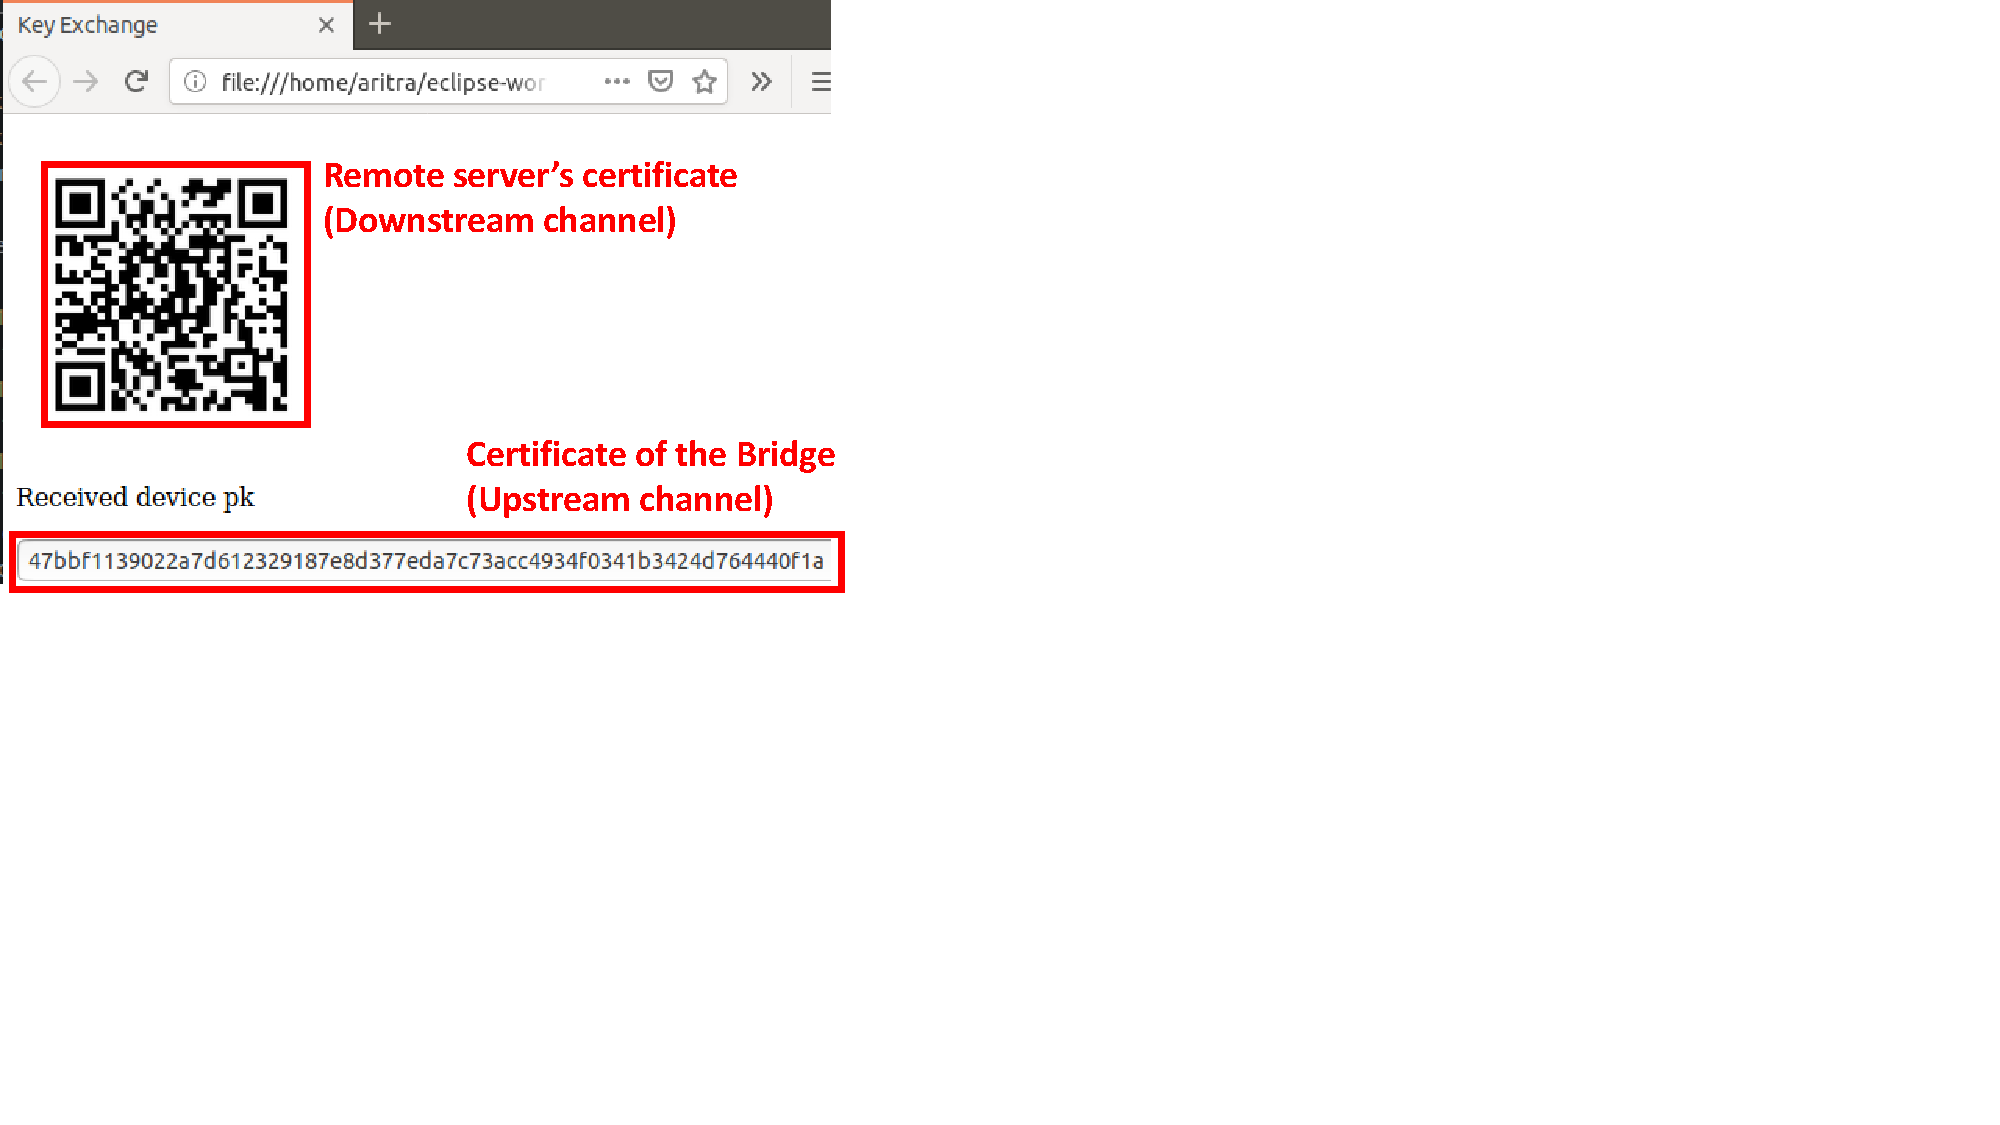
\includegraphics[trim={0 8cm 18cm 0}, clip, width=0.85\linewidth]{keyExchange.pdf}
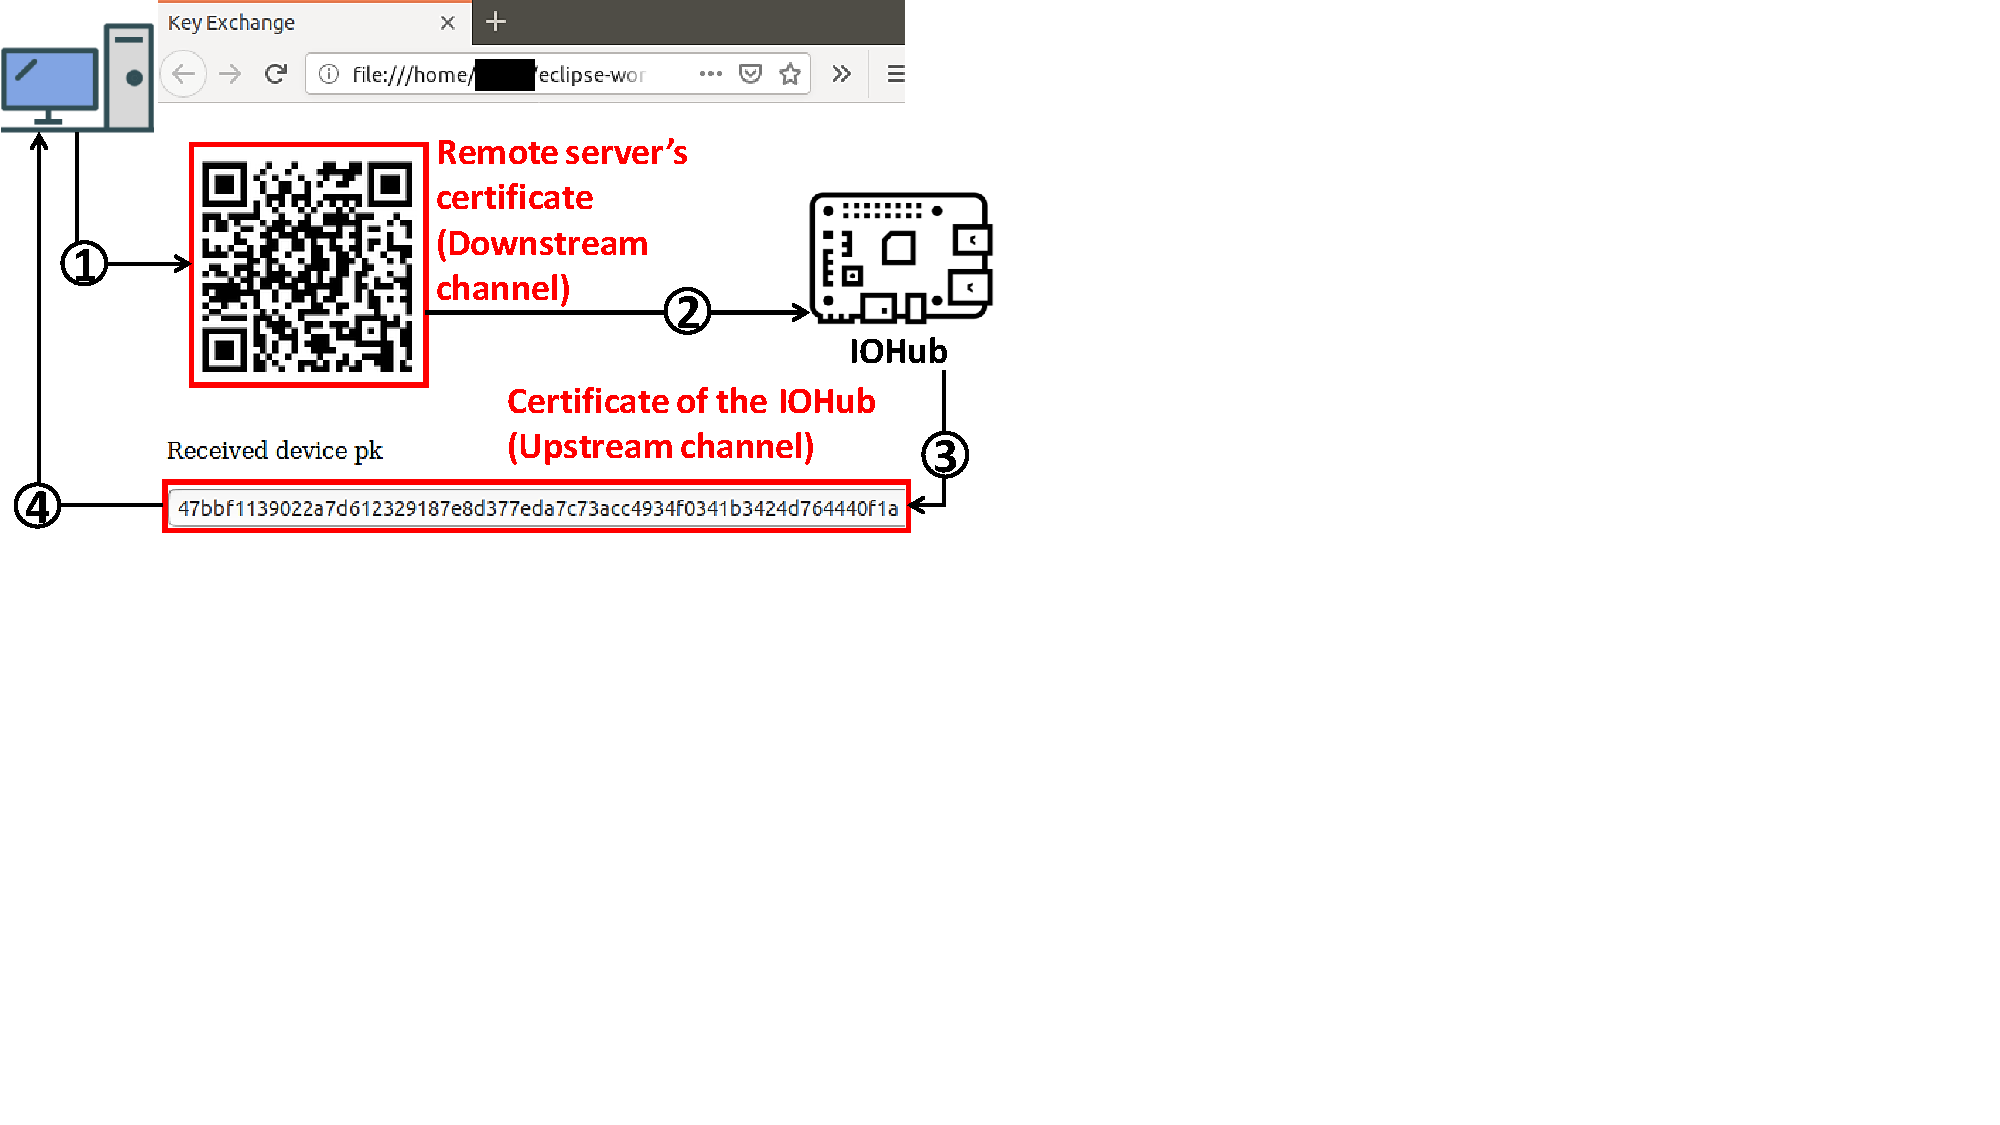
\includegraphics[trim={0 10cm 17cm 0}, clip, width=0.85\linewidth]{keyExchange_1.pdf}
\caption{\textbf{Establishing \tls.} A snapshot of the key exchange web page that is used to communicate the public certificates of the device and the remote server. This page only lasts for a few milliseconds. Hence the page is practically invisible to the user. The QR-code displayed on the web page serves as the downstream channel from the remote server to the \device, whereas the text field is the upstream channel.}
\spacesave
\label{fig:keyExchange}
\centering
\end{figure} 

%Note that as described in the system model (see Section~\ref{sec:approach:systemAttackerModel}), the \device lacks any network capability. Hence 
Remember that the \device relies on the untrusted host as the communication channel as it lacks any network capability (refer to Section~\ref{sec:approach:systemAttackerModel}). The \device and the remote server have a bidirectional channel. The downstream channel is the encoded UI specification (see Section~\ref{sec:systemDesign:transformation}) sent by the server and the \name \js provides the upstream channel (see Section~\ref{sec:systemDesign:commit:upload}). 
When the user opens up a webpage that supports \name mechanism, key exchange is the first step that is executed by the \device. Also, the key exchange phase is crucial as the remote server also decide if the user has a \device. We assume that the remote server already has the \device's certificate, or some offline registration takes place. An instance of the key exchange mechanism of \name is illustrated in Figure~\ref{fig:keyExchange}. The flow of the key exchange mechanism is as the following:

\begin{mylist}
  \item[\one] The remote web server serves the web page that shows a QR code that encodes the signed public key of the remote server (server hello in TLS). This page has a $5$ seconds timeout.
  \item[\two] The device captures the frames and looks for a QR code. As soon as the device finds one, the device decodes the QR code and verifies it. If the verification is successful, the device emulates itself as a keyboard device to the host system. The device then encodes its signed public certificate to hexadecimal and send it as a keystroke to the host (client hello in the TLS). For signature, the \device uses the root key of the device manufacturer.
  \item[\three] \name  JavaScript snippet looks for the keystrokes, and as soon as it gets a string of a specific length, it sends the key strokes to the remote server.
  \item[\four] The remote server gets the signed certificate from the \device,. If the verification is successful, the server derives the shared secret.
 
\end{mylist}

After this, both the device and the remote server have each other's public
certificates. Using these certificates, both the \device and remote server
calculates the shared secret using the authenticated Diffie-Hellman
protocol~\cite{blake1998authenticated}.
%~\footnote{Assume that $(g^x, x)$ and $(g^y, y)$ is the public-private key pair of the remote server and the \device respectively, where $g$ being a generator of a group $G$. The remote server sends a QR code that encodes a CA-signed $g^x$. The \device transmits signed $g^y$ to the remote server. Both the remote server and the \device computes $g^{xy}=(g^x)^y=(g^y)^x$ as the shared secret. Detailed description can be found  in~\cite{blake1998authenticated}.}.
In the case the user does not have a \device, the step mentioned above does not take place within the $5$ seconds timeout period. In that case, \name JavaScript snippet concludes that the user does not have a \device. This allows the webpage to fallback to conventional web UIs that do not involve \device for their operation.


